\documentclass[conference]{IEEEtran}
\IEEEoverridecommandlockouts
%Template version as of 6/27/2024

\usepackage[utf8]{inputenc}
\usepackage[T1]{fontenc}
\usepackage{cite}
\usepackage{amsmath,amssymb,amsfonts}
\usepackage{algorithmic}
\usepackage{graphicx}
\usepackage{textcomp}
\usepackage{xcolor}
\graphicspath{
  {../reports/figures/}
  {../reports/figures/eda/}
  {../reports/figures/comparacion/}
  {../reports/results/}
  {../reports/results/image_comparison/}
}
\def\BibTeX{{\rm B\kern-.05em{\sc i\kern-.025em b}\kern-.08em
    T\kern-.1667em\lower.7ex\hbox{E}\kern-.125emX}}
\begin{document}

\title{Detección de humo y fuego mediante arquitecturas profundas de detección de objetos}

\author{\IEEEauthorblockN{1\textsuperscript{st} Given Name Surname}
\IEEEauthorblockA{\textit{dept. name of organization (of Aff.)} \\
\textit{name of organization (of Aff.)}\\
City, Country \\
email address or ORCID}
\and
\IEEEauthorblockN{2\textsuperscript{nd} Given Name Surname}
\IEEEauthorblockA{\textit{dept. name of organization (of Aff.)} \\
\textit{name of organization (of Aff.)}\\
City, Country \\
email address or ORCID}
\and
\IEEEauthorblockN{3\textsuperscript{rd} Given Name Surname}
\IEEEauthorblockA{\textit{dept. name of organization (of Aff.)} \\
\textit{name of organization (of Aff.)}\\
City, Country \\
email address or ORCID}
\and
\IEEEauthorblockN{4\textsuperscript{th} Given Name Surname}
\IEEEauthorblockA{\textit{dept. name of organization (of Aff.)} \\
\textit{name of organization (of Aff.)}\\
City, Country \\
email address or ORCID}
\and
\IEEEauthorblockN{5\textsuperscript{th} Given Name Surname}
\IEEEauthorblockA{\textit{dept. name of organization (of Aff.)} \\
\textit{name of organization (of Aff.)}\\
City, Country \\
email address or ORCID}
\and
\IEEEauthorblockN{6\textsuperscript{th} Given Name Surname}
\IEEEauthorblockA{\textit{dept. name of organization (of Aff.)} \\
\textit{name of organization (of Aff.)}\\
City, Country \\
email address or ORCID}
}

\maketitle

\begin{abstract}
La detección temprana de humo y fuego constituye una aplicación relevante
de la visión por computadora debido a la necesidad de identificar
situaciones potencialmente peligrosas de forma rápida y automática. En este
trabajo se aborda este problema con el conjunto de datos D-Fire, compuesto
por 21\,527 imágenes que contienen humo, fuego, ambas clases
simultáneamente y escenas negativas. Sobre las mismas particiones de datos
se entrenan y evalúan cinco arquitecturas que representan tres paradigmas de
detección: YOLOv8n, YOLO11n y YOLO26s (una etapa), Faster R-CNN (dos etapas)
y RT-DETR-L (Transformer end-to-end).

Los cinco modelos alcanzan un desempeño comparable sobre el conjunto de
validación (mAP@0.5 entre 0.757 y 0.778), con diferencias de velocidad de
inferencia de hasta un factor 60. Los resultados indican que la calidad de
las anotaciones y el tamaño de los objetos condicionan el desempeño más que
la elección de la arquitectura, y que los modelos livianos de una etapa
ofrecen el mejor compromiso entre detección y costo computacional.
\end{abstract}

\begin{IEEEkeywords}
detección de objetos, humo, fuego, visión por computadora, aprendizaje profundo,
YOLO, Faster R-CNN, RT-DETR.
\end{IEEEkeywords}

\section{Introducción}
La detección temprana de incendios constituye un problema de importancia en
sistemas de monitoreo, seguridad y prevención de riesgos: una identificación
rápida de la presencia de humo o fuego contribuye a reducir los tiempos de
respuesta y limitar sus consecuencias.

Los sistemas tradicionales de detección suelen utilizar sensores físicos de
temperatura, humo o partículas, que requieren que los efectos del incendio
alcancen físicamente al sensor para generar una alarma. El análisis
automático de imágenes representa una alternativa complementaria que permite
detectar evidencias visuales de un posible incendio a partir de cámaras de
monitoreo. Los avances en aprendizaje profundo han permitido que los
detectores de objetos aprendan automáticamente las representaciones
visuales necesarias, sin diseñar manualmente características de color,
textura o forma.

Existen diferentes estrategias para abordar el problema de detección de
objetos. Los modelos de la familia YOLO realizan la detección mediante una
arquitectura de una etapa, estimando directamente las clases y las cajas
delimitadoras \cite{b1}, lo que les otorga una elevada velocidad de
inferencia. Faster R-CNN utiliza en cambio un esquema de dos etapas: una
Region Proposal Network genera regiones candidatas que luego son
clasificadas y refinadas \cite{b2}. Más recientemente, RT-DETR propone una
arquitectura end-to-end basada en Transformers, orientada a combinar las
capacidades de los modelos DETR con una velocidad de procesamiento adecuada
para aplicaciones en tiempo real \cite{b3}.

En este trabajo se estudia la detección automática de humo y fuego sobre el
conjunto de datos D-Fire \cite{b4}. Se entrenan cinco arquitecturas
(YOLOv8n, YOLO11n, YOLO26s, Faster R-CNN y RT-DETR-L) sobre las mismas
particiones de datos y se comparan bajo un protocolo experimental común, con
métricas estándar de detección y medidas de eficiencia computacional.


\section{Estado del arte}

Un antecedente directo de este proyecto es el sistema propuesto por
Venâncio \textit{et al.} \cite{b4}, desarrollado en el contexto de un
sistema de videovigilancia para detección temprana de incendios en Brasil.
Los autores abordaron el mismo problema que se estudia aquí, la detección de
humo y fuego en imágenes de cámaras de monitoreo mediante detectores de
objetos, con la restricción adicional de que el sistema debía ejecutarse en
dispositivos de bajo consumo y recursos limitados. Para ello evaluaron
variantes de la familia YOLOv4, incluyendo versiones comprimidas de la red,
y midieron el compromiso entre capacidad de detección y tiempo de
inferencia en hardware embebido. Una de sus conclusiones principales es que
los modelos convolucionales compactos alcanzan un desempeño competitivo
frente a variantes de mayor tamaño, con tiempos de inferencia compatibles
con la operación en tiempo real sobre dispositivos de bajo costo. Como parte
de ese trabajo construyeron y publicaron el conjunto de datos D-Fire, con
más de 21\,000 imágenes anotadas, que es el que se utiliza en el presente
estudio.

Este trabajo puede situarse como una extensión natural de ese antecedente:
mientras que en \cite{b4} se comparan variantes de una única familia de
detectores, aquí se contrastan sobre el mismo conjunto de datos tres
paradigmas arquitectónicos surgidos con posterioridad.


\section{Materiales y métodos}

\subsection{Dataset D-Fire}\label{dataset}
Para el desarrollo del trabajo se utiliza el conjunto de datos D-Fire
\cite{b4}, diseñado específicamente para el entrenamiento y evaluación de
sistemas automáticos de detección de humo y fuego.

El conjunto de datos contiene imágenes pertenecientes a cuatro tipos de
escenas: imágenes que contienen únicamente fuego, imágenes que contienen
únicamente humo, imágenes en las que ambos fenómenos aparecen
simultáneamente y escenas negativas que no contienen ninguna de las dos
clases. La Fig.~\ref{fig:muestra_dataset} presenta una muestra aleatoria del
conjunto de datos con ejemplos de las cuatro categorías.

\begin{figure*}[!t]
\centerline{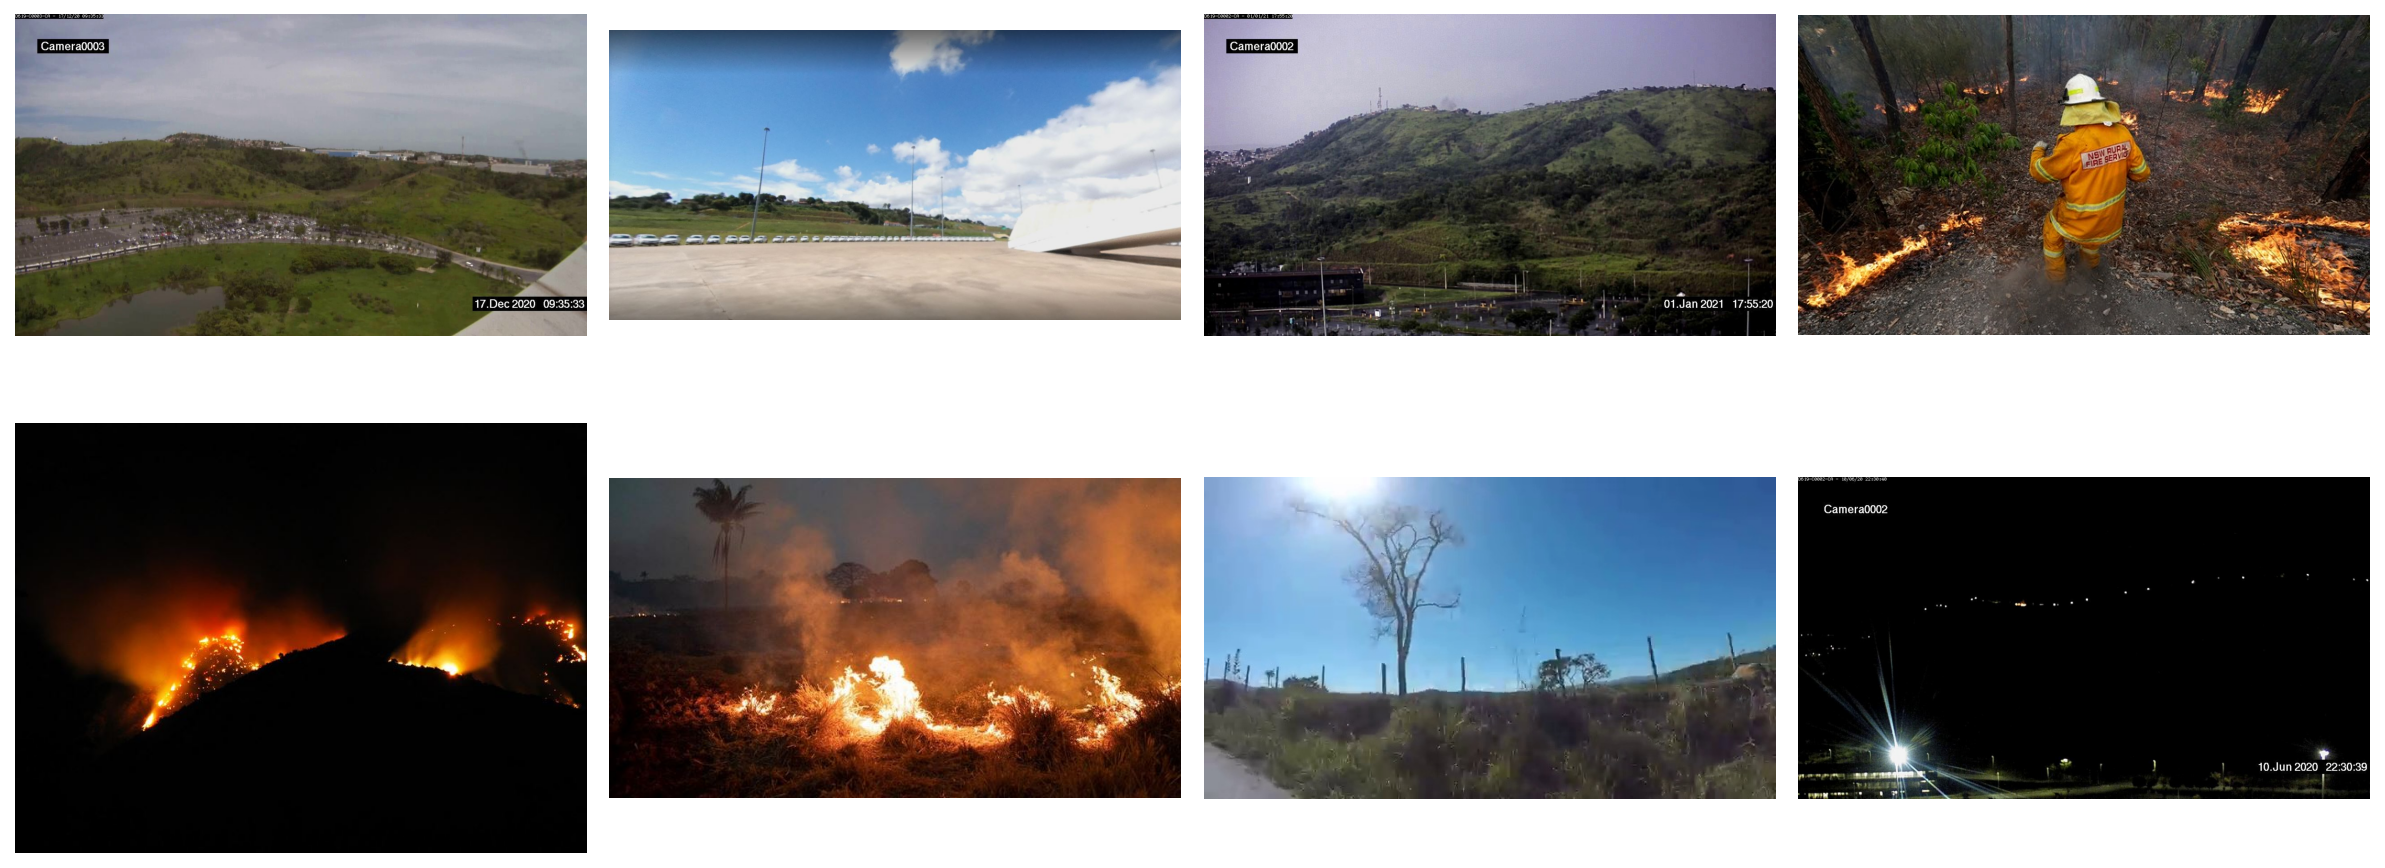
\includegraphics[width=0.88\textwidth]{muestra_dataset.png}}
\caption{Muestra aleatoria de ocho imágenes de D-Fire con ejemplos de las
cuatro categorías de escena. Se observa la diversidad de fuentes (cámaras
fijas de vigilancia, fotografías a nivel de suelo), de iluminación y de
escala de los fenómenos.}
\label{fig:muestra_dataset}
\end{figure*}

La inclusión de imágenes negativas es particularmente relevante para este
problema debido a que expone a los modelos durante el entrenamiento a
escenas sin eventos de interés, incluyendo fondos visualmente similares al
humo como nubes o niebla. Las anotaciones se representan mediante cajas
delimitadoras con dos clases: \textit{smoke} (regiones de humo) y
\textit{fire} (regiones de fuego).

El conjunto completo utilizado en el proyecto está compuesto por 21\,527
imágenes. Para mantener un protocolo experimental común se conserva la
partición original del conjunto de datos en subconjuntos de entrenamiento,
validación y test, cuya distribución se presenta en la
Tabla~\ref{tab:dataset_split}.

\begin{table}[htbp]
\caption{Distribución del conjunto de datos D-Fire}
\begin{center}

\begin{tabular}{|c|c|}
\hline

\textbf{Partición} &
\textbf{Cantidad de imágenes} \\

\hline

Entrenamiento & 14\,122 \\

\hline

Validación & 3\,099 \\

\hline

Test & 4\,306 \\

\hline

Total & 21\,527 \\

\hline

\end{tabular}

\label{tab:dataset_split}

\end{center}
\end{table}

El conjunto de entrenamiento se utiliza para ajustar los modelos, el de
validación para compararlos y seleccionar el mejor punto de control, y el de
test se reserva para la evaluación cualitativa de la
Sección~\ref{sec:cualitativa}.

Cabe una aclaración sobre la composición del conjunto: una parte sustancial
de las imágenes proviene de cámaras fijas que registraron la misma escena en
distintos instantes, es decir, series temporales guardadas como imágenes
individuales. La partición original se realizó a nivel de imagen, sin
agrupar por cámara ni por secuencia, por lo que imágenes casi idénticas
pueden aparecer en particiones distintas. Se decidió conservarla de todos
modos porque mantiene la comparabilidad con otros trabajos y porque el
dataset no provee metadatos para reconstruir las secuencias. Como
contrapartida, las métricas reportadas deben interpretarse como una cota
optimista de la generalización a escenas completamente nuevas.

\subsection{Análisis exploratorio y preparación de datos}\label{Preparacion_datos}
Antes del entrenamiento se realizó una exploración del conjunto de datos con
el objetivo de verificar la estructura de las carpetas, la correspondencia
entre imágenes y archivos de etiquetas, la validez de las anotaciones y la
distribución de clases. Las imágenes y etiquetas se encuentran organizadas
en la estructura estándar de YOLO (\texttt{images} y \texttt{labels} por
partición), donde cada objeto se representa mediante la clase y las
coordenadas normalizadas de su caja delimitadora.

\begin{figure}[htbp]
\centerline{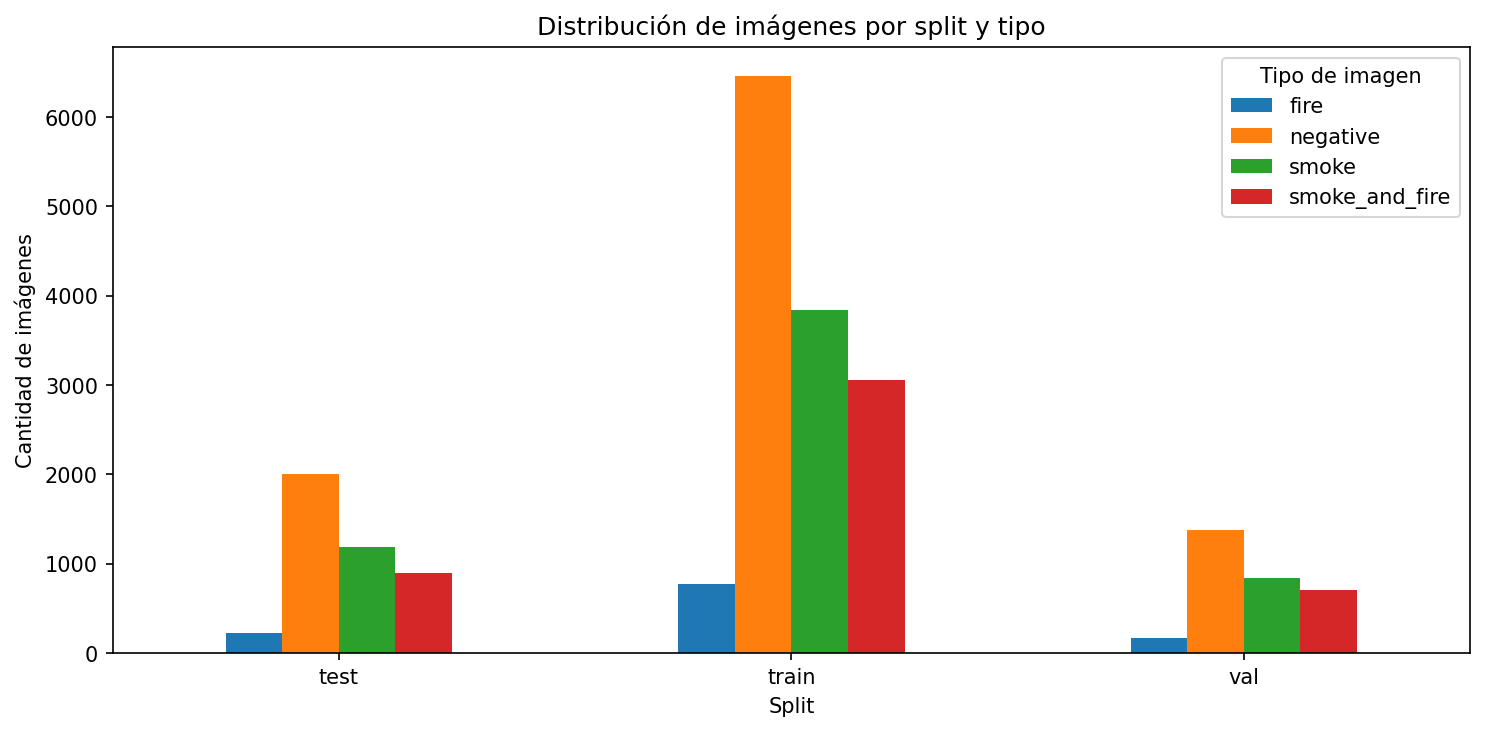
\includegraphics[width=0.85\columnwidth]{image_type_distribution.png}}
\caption{Distribución de imágenes por partición según el tipo de escena.
Las escenas negativas son la categoría mayoritaria en las tres particiones,
mientras que las imágenes con fuego únicamente son minoritarias.}
\label{fig:image_types}
\end{figure}

La Fig.~\ref{fig:image_types} muestra la distribución de tipos de escena por
partición. Las imágenes negativas son la categoría más numerosa (9\,838
imágenes, el 46\% del total), mientras que las imágenes que contienen
únicamente fuego son escasas (1\,164 imágenes, el 5\%). Este desbalance
aparente se atenúa al analizar las anotaciones a nivel de objeto: como el
fuego aparece mayormente acompañado de humo, la cantidad total de cajas es
similar entre clases (14\,692 de \textit{fire} frente a 11\,865 de
\textit{smoke}). Por este motivo no se aplicó ninguna estrategia de
rebalanceo de clases. Las imágenes negativas se conservaron en su totalidad
dado que exponen al detector a fondos difíciles y contribuyen a reducir los
falsos positivos, efecto que se verifica en la evaluación cualitativa.

\begin{figure}[htbp]
\centerline{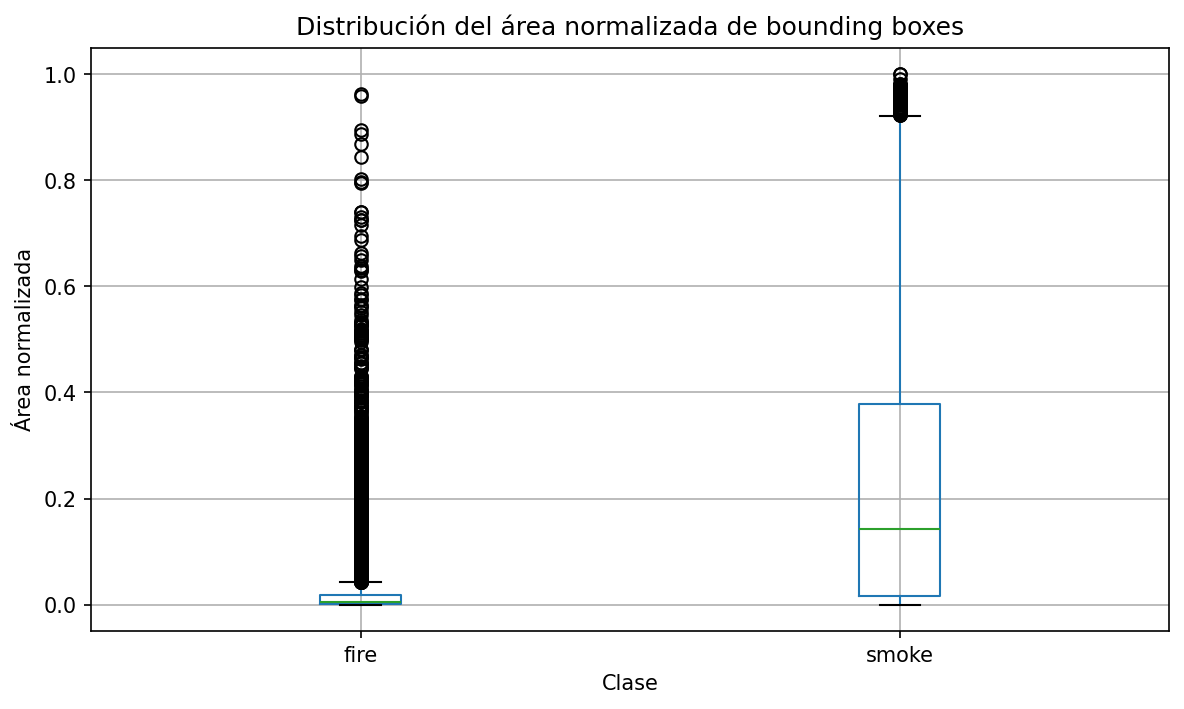
\includegraphics[width=0.85\columnwidth]{bbox_area_distribution.png}}
\caption{Distribución del área normalizada de las cajas delimitadoras por
clase. Las cajas de \textit{fire} se concentran en áreas muy pequeñas
(mediana inferior al 2\% de la imagen), mientras que las de \textit{smoke}
son en general más grandes y presentan mayor dispersión.}
\label{fig:bbox_areas}
\end{figure}

La Fig.~\ref{fig:bbox_areas} presenta la distribución del área normalizada
de las cajas por clase. La mayoría de las cajas de \textit{fire} comparte un
tamaño pequeño, con mediana inferior al 2\% del área de la imagen, mientras
que las de \textit{smoke} son considerablemente más grandes, con una
distribución más extendida. Esta asimetría anticipa que la clase
\textit{fire} plantea un problema de detección de objetos pequeños, aspecto
que se retoma en el análisis de resultados.

La validación de anotaciones detectó únicamente 8 cajas del conjunto de test
con coordenadas levemente fuera del rango normalizado $[0,1]$, sobre más de
26\,000 cajas; dado su volumen marginal y que los marcos de entrenamiento
recortan las coordenadas al rango válido, no fueron modificadas. Durante la
inspección visual se identificaron además errores de anotación de origen
(etiquetas intercambiadas entre clases y objetos sin anotar); corregirlos
habría requerido re-anotar manualmente el conjunto completo, por lo que se
decidió no intervenir el dataset. Su efecto sobre las métricas se discute en
la Sección~\ref{sec:cualitativa}.

\subsection{Modelos de detección de objetos}


Se seleccionaron cinco modelos que cubren tres paradigmas de detección de
objetos: detectores de una etapa (YOLOv8n, YOLO11n y YOLO26s), de dos etapas
(Faster R-CNN) y basados en Transformers (RT-DETR-L).

% ============================================================
% C.1 YOLOV8
% ============================================================

\subsubsection{YOLOv8n}

YOLOv8n \cite{b5} se utiliza como modelo de referencia o \textit{baseline}
del proyecto. La variante nano corresponde a una de las configuraciones más
livianas de la familia YOLOv8 y establece el punto de comparación para las
arquitecturas restantes.

% ============================================================
% C.2 YOLO11
% ============================================================

\subsubsection{YOLO11n}

YOLO11n corresponde a una generación posterior de la familia YOLO. Se utiliza
también su variante nano con el objetivo de evaluar si las modificaciones
arquitectónicas introducidas respecto de generaciones anteriores permiten
obtener mejoras manteniendo un bajo costo computacional.

% ============================================================
% C.3 YOLO26
% ============================================================

\subsubsection{YOLO26s}

YOLO26s corresponde a la variante small de una generación posterior de la
familia YOLO. A diferencia de las variantes nano anteriores, en este caso se
utiliza un modelo de mayor capacidad, con el objetivo de estudiar si un
incremento moderado en la complejidad mejora la detección sin recurrir a las
variantes de mayor tamaño de la arquitectura.

% ============================================================
% C.4 FASTER R-CNN
% ============================================================

\subsubsection{Faster R-CNN}

Faster R-CNN emplea una estrategia de dos etapas: una Region Proposal
Network genera regiones candidatas que luego son clasificadas y refinadas
\cite{b2}. Se utiliza una implementación basada en un backbone ResNet-50 con
Feature Pyramid Network.

% ============================================================
% C.5 RT-DETR
% ============================================================

\subsubsection{RT-DETR-L}

RT-DETR pertenece a una familia de detectores basados en Transformers,
desarrollada para permitir detección end-to-end manteniendo velocidades de
procesamiento adecuadas para aplicaciones en tiempo real \cite{b3}. Se
utiliza la variante RT-DETR-L.


\subsection{Protocolo experimental}

Cada entrenamiento se encuentra asociado a un archivo de configuración
versionado en el repositorio del proyecto, que define la arquitectura, los
pesos iniciales, las épocas, los tamaños de imagen y de \textit{batch}, el
optimizador, la tasa de aprendizaje, el criterio de \textit{early stopping}
y la semilla aleatoria. Los cinco modelos comparten idénticas particiones de
datos, resolución de entrada de $640 \times 640$ píxeles y semilla fija.
Todos parten de pesos preentrenados sobre COCO: en los modelos
implementados con Ultralytics \cite{b5} se ajusta la red completa, mientras
que en Faster R-CNN se ajustan el cabezal de detección y las últimas tres
etapas del backbone.

Debido al elevado costo computacional de los entrenamientos, que insumieron
entre 4 y 18.5 horas por corrida sobre una GPU Tesla T4, no se realizó una
búsqueda sistemática de hiperparámetros: cada arquitectura se entrenó una
única vez, con configuraciones cercanas a los valores por defecto de su
implementación de referencia. Los modelos YOLO se entrenaron durante 50
épocas con los hiperparámetros por defecto de Ultralytics y \textit{early
stopping} por paciencia; Faster R-CNN con la receta estándar de torchvision
(SGD con momento 0.9, tasa inicial 0.005 y decaimiento coseno). La única
desviación deliberada corresponde a RT-DETR-L, donde se fijó AdamW con tasa
$10^{-4}$ porque la selección automática de Ultralytics asignaba una
configuración de SGD inadecuada para un Transformer. Faster R-CNN y
RT-DETR-L se entrenaron 30 épocas en lugar de 50 para igualar
aproximadamente el presupuesto de cómputo y no favorecer a los modelos de
mayor costo por época; como se muestra en la
Sección~\ref{sec:entrenamiento}, ambos alcanzan su meseta dentro de ese
presupuesto.

De cada experimento se selecciona el punto de control con mejor mAP@0.5:0.95
sobre validación y se versionan los pesos, curvas de entrenamiento, métricas
y matrices de confusión. La comparación cuantitativa se realiza sobre el
conjunto de validación, mientras que el de test se reserva para la
evaluación cualitativa.


% ============================================================
% E. MÉTRICAS
% ============================================================

\subsection{Métricas de evaluación}

La evaluación se realiza con métricas estándar de detección de objetos. La
precisión y el recall se definen como

\begin{equation}
Precision = \frac{TP}{TP+FP}, \qquad
Recall = \frac{TP}{TP+FN},
\label{eq:precision_recall}
\end{equation}

donde $TP$, $FP$ y $FN$ representan los verdaderos positivos, falsos
positivos y falsos negativos, respectivamente. El F1-score las considera
simultáneamente:

\begin{equation}
F1 =
2
\frac{Precision \cdot Recall}
{Precision + Recall}.
\label{eq:f1}
\end{equation}

Para evaluar conjuntamente la clasificación y la localización se utiliza la
mean Average Precision (mAP), en sus variantes $mAP@0.50$ (umbral de
Intersection over Union de 0.50) y $mAP@0.50:0.95$ (promedio sobre umbrales
entre 0.50 y 0.95). Se adopta $mAP@0.50:0.95$ como métrica principal de
comparación, dado que penaliza las localizaciones imprecisas. Además, se
mide la velocidad de inferencia en imágenes por segundo (FPS) sobre una GPU
Tesla T4, para estudiar el compromiso entre desempeño y costo
computacional.


% ============================================================
% III. RESULTADOS
% ============================================================

\section{Resultados}\label{sec:resultados}

\subsection{Comparación cuantitativa}

La Tabla~\ref{tab:metricas} resume las métricas obtenidas por cada modelo
sobre el conjunto de validación, evaluadas en el mejor punto de control de
cada entrenamiento.

\begin{table}[htbp]
\caption{Métricas de detección sobre el conjunto de validación}
\begin{center}
\begin{tabular}{|l|c|c|c|c|c|}
\hline
\textbf{Modelo} & \textbf{P} & \textbf{R} & \textbf{F1} &
\textbf{mAP@0.5} & \textbf{mAP@0.5:0.95} \\
\hline
YOLOv8n      & 0.780 & 0.691 & 0.733 & 0.771 & 0.447 \\
\hline
YOLOv11n      & 0.776 & 0.693 & 0.732 & 0.761 & 0.445 \\
\hline
YOLO26s      & 0.775 & 0.714 & 0.743 & \textbf{0.778} & \textbf{0.459} \\
\hline
Faster R-CNN & \textbf{0.800} & \textbf{0.726} & \textbf{0.761} & 0.769 & 0.424 \\
\hline
RT-DETR-L    & 0.745 & 0.705 & 0.725 & 0.757 & 0.430 \\
\hline
\end{tabular}
\label{tab:metricas}
\end{center}
\end{table}

El primer resultado destacable es la homogeneidad de los valores: el rango de
mAP@0.5 entre el mejor y el peor modelo es de apenas 2.1 puntos porcentuales
(0.757 a 0.778) y el de mAP@0.5:0.95 de 3.5 puntos (0.424 a 0.459). Cinco
arquitecturas que difieren en paradigma y en más de un orden de magnitud de
tamaño (de 2.6 a 43.3 millones de parámetros) convergen a un desempeño casi
indistinguible, lo que sugiere que el techo está determinado por las
características del conjunto de datos (objetos pequeños, límites difusos del
humo y errores de anotación) más que por la capacidad de los modelos.

Dentro de ese rango acotado se observan dos comportamientos diferenciados.
YOLO26s obtiene los mejores valores de mAP en ambos umbrales (0.778 y 0.459),
consistente con ser el YOLO de mayor capacidad evaluado. Faster R-CNN, en
cambio, lidera precisión (0.800), recall (0.726) y F1 (0.761) pero registra el
peor mAP@0.5:0.95 (0.424): su punto de operación clasifica y detecta bien,
pero sus cajas pierden solapamiento frente a las de los YOLO cuando el
criterio de IoU se vuelve más exigente. Dado que cada arquitectura se entrenó
una única vez, estas diferencias menores deben interpretarse como indicativas
y no como estadísticamente significativas.

El desglose por clase es consistente entre modelos y resulta más informativo
que las diferencias entre arquitecturas: el mAP@0.5 de \textit{smoke} se
ubica entre 0.798 y 0.828 y el de \textit{fire} entre 0.709 y 0.725, una
brecha de unos 10 puntos que ningún modelo logra cerrar. Esta dificultad
estructural se explica por el análisis exploratorio de la
Fig.~\ref{fig:bbox_areas}: las cajas de fuego son mayoritariamente muy
pequeñas, y la detección de objetos pequeños es una limitación conocida de
los detectores evaluados a resolución de entrada moderada.

Las matrices de confusión refuerzan este diagnóstico: la confusión entre
clases es prácticamente nula (del orden del 1\% en YOLOv8n, con un patrón
análogo en el resto), de modo que el error dominante no es clasificar mal un
objeto detectado sino omitirlo (el 21\% de las instancias de humo y el 29\%
de las de fuego en YOLOv8n). Para un sistema de alerta temprana este es el
tipo de error más costoso, por lo que mejorar el recall constituye la
principal línea de mejora.

\subsection{Análisis del entrenamiento}\label{sec:entrenamiento}

La evolución por época de las métricas de validación revela dinámicas de
convergencia muy distintas entre paradigmas: Faster R-CNN parte desde la
primera época con un mAP@0.5 cercano a 0.69, dado que su backbone
preentrenado y su esquema de propuestas transfieren de inmediato al nuevo
dominio, mientras que YOLOv8n comienza en torno a 0.25 y RT-DETR-L por
debajo de 0.05, con el arranque lento característico de los Transformers.
Hacia el final del entrenamiento las curvas convergen a valores
prácticamente indistinguibles, lo que confirma que el presupuesto de épocas
fue suficiente para todos los paradigmas y respalda la observación anterior:
ninguna arquitectura supera de manera sostenida el techo común. YOLO26s
alcanzó su mejor punto de control en la época 40 de 50, con las métricas ya
en meseta.

\subsection{Compromiso entre desempeño y velocidad}

La Tabla~\ref{tab:eficiencia} resume el costo computacional de cada modelo.
Dado que las métricas de detección son casi equivalentes, la eficiencia se
convierte en el principal criterio de selección práctica.

\begin{table}[htbp]
\caption{Eficiencia computacional (GPU Tesla T4)}
\begin{center}
\begin{tabular}{|l|c|c|c|c|}
\hline
\textbf{Modelo} & \textbf{Parám. (M)} & \textbf{Épocas} &
\textbf{Entren. (min)} & \textbf{FPS} \\
\hline
YOLOv8n      & 3.0  & 50 & 243  & \textbf{455.0} \\
\hline
YOLOv11n      & 2.6  & 50 & 251   & 359.46   \\
\hline
YOLO26s      & 10.0 & 50 & 314  & 188.0 \\
\hline
Faster R-CNN & 43.3 & 30 & 1112 & 7.4  \\
\hline
RT-DETR-L    & 32.0 & 30 & 563  & 26.9 \\
\hline
\end{tabular}
\label{tab:eficiencia}
\end{center}
\end{table}

El contraste es marcado: YOLOv8n procesa 455 imágenes por segundo, 60 veces
más que Faster R-CNN (7.4 FPS), y sin embargo lo iguala o supera en mAP
(0.771 frente a 0.769 en mAP@0.5 y 0.447 frente a 0.424 en mAP@0.5:0.95). La
ventaja de Faster R-CNN en F1 (+2.9 puntos sobre YOLOv8n) podría justificar
su uso únicamente en procesamiento diferido; su costo de entrenamiento
también es muy superior (18.5 frente a 4 horas). YOLO26s ofrece un punto
intermedio atractivo: el mejor mAP de la comparación manteniendo 188 FPS.
Para el caso de uso que motiva este trabajo, el monitoreo simultáneo de
múltiples cámaras en tiempo real, los modelos YOLO dominan claramente el
compromiso desempeño-velocidad.

\subsection{Evaluación cualitativa}\label{sec:cualitativa}

Para complementar las métricas se comparan las predicciones de los cinco
modelos sobre imágenes del conjunto de test, que no participó del
entrenamiento ni de la selección de puntos de control.

Un primer patrón recurrente aparece en las escenas con múltiples focos: las
variantes nano de las generaciones YOLO más antiguas (YOLOv8n y YOLO11n)
recuperan solo la instancia principal de fuego, mientras que YOLO26s detecta
varios focos y Faster R-CNN y RT-DETR-L capturan también los secundarios (en
un caso representativo con seis objetos anotados, una única detección frente
a ocho). Esto es coherente con la Tabla~\ref{tab:metricas}, donde ambos
nano registran el recall más bajo (0.691) y Faster R-CNN el más alto
(0.726).

\begin{figure*}[!t]
\centerline{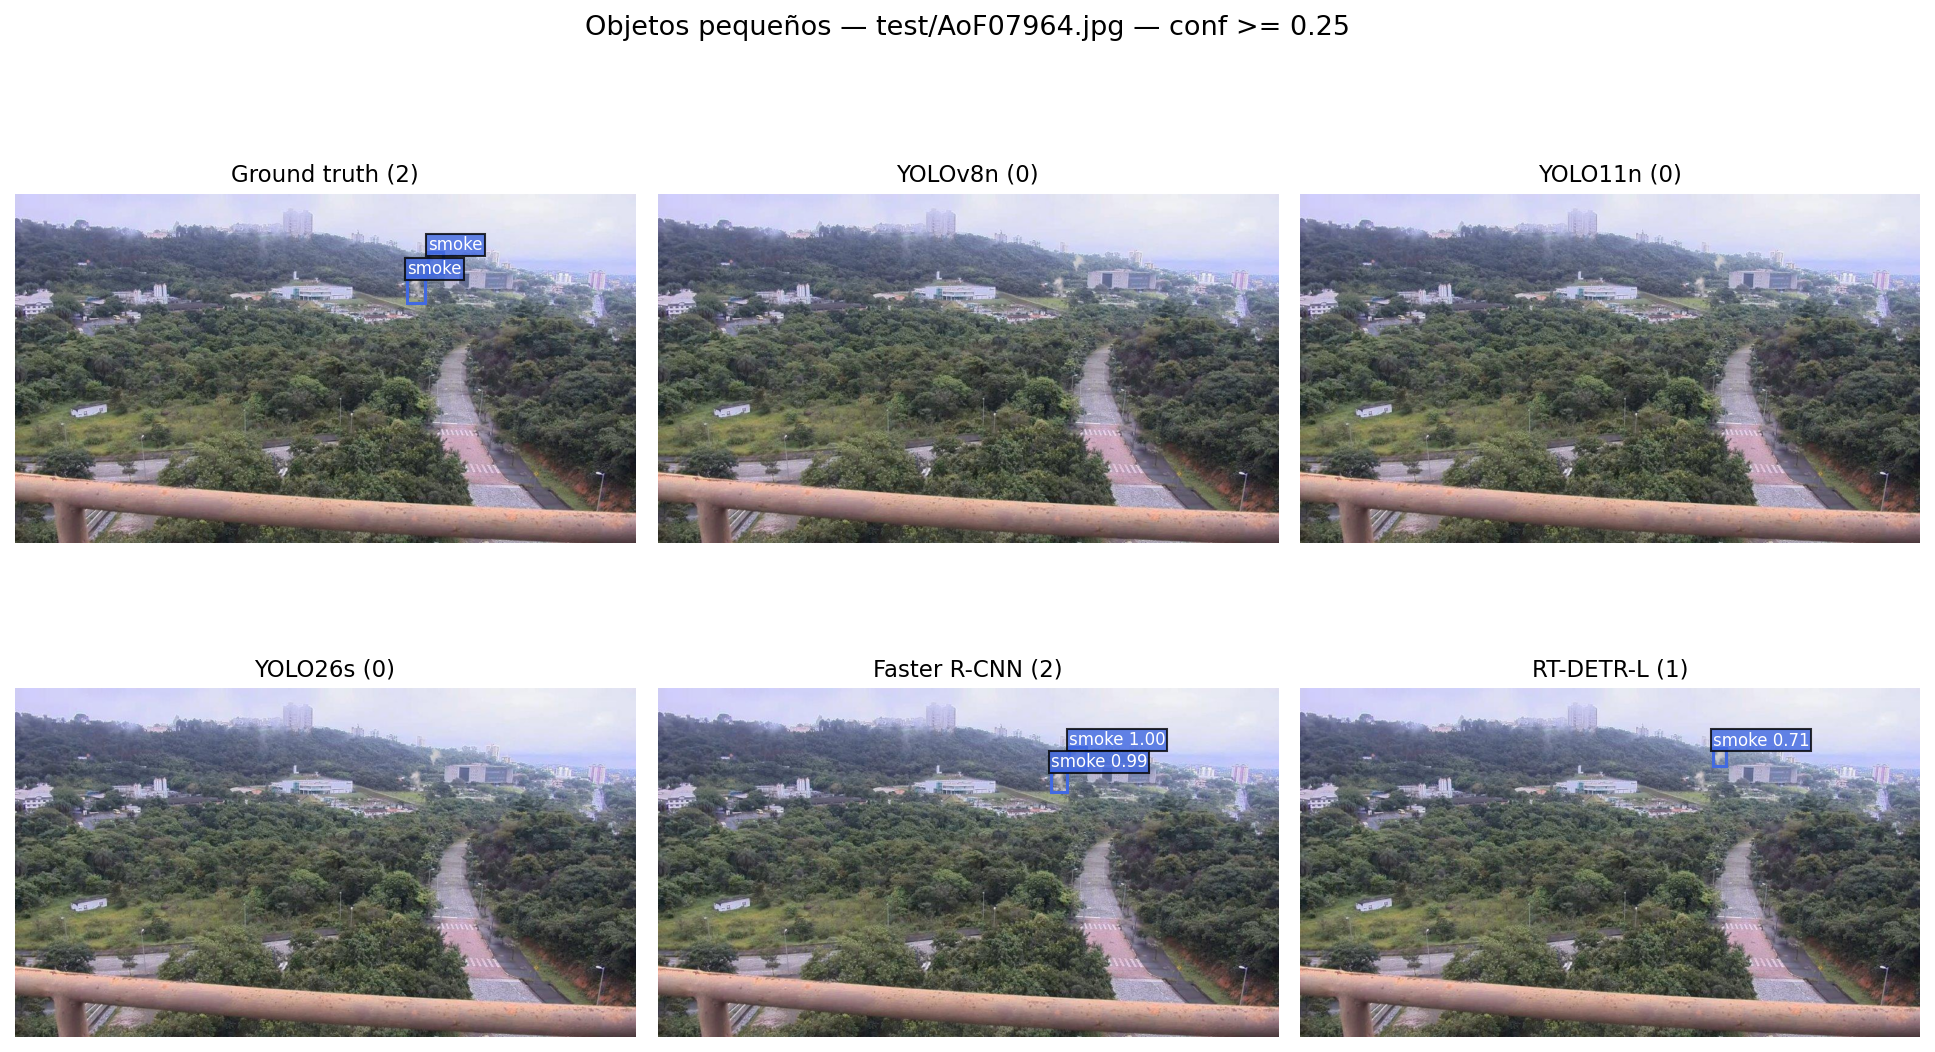
\includegraphics[width=0.7\textwidth]{cualitativa_objetos_pequenos_AoF07964.png}}
\caption{Escena con objetos pequeños (test/AoF07964, confianza $\geq 0.25$):
dos columnas de humo distantes que ocupan menos del 1\% de la imagen. Los
tres modelos YOLO no producen ninguna detección, RT-DETR-L recupera una de
las dos instancias y Faster R-CNN recupera ambas con confianza cercana a 1.0.}
\label{fig:cualitativa_pequenos}
\end{figure*}

El caso más diferenciador es el de los objetos pequeños
(Fig.~\ref{fig:cualitativa_pequenos}): frente a columnas de humo lejanas que
ocupan menos del 1\% de la imagen, los tres modelos YOLO no detectan ninguna
instancia, RT-DETR-L recupera una y Faster R-CNN recupera las dos con
confianza cercana a 1.0. Una explicación plausible es que las variantes nano
y small evaluadas carecen de la capacidad necesaria, mientras que la
pirámide de características con propuestas densas de Faster R-CNN retiene
mejor la evidencia de objetos diminutos. Este caso concentra la brecha de
recall señalada en las matrices de confusión y es crítico para la
aplicación, dado que un foco lejano y pequeño es precisamente el evento que
un sistema de alerta temprana debe capturar.

En las imágenes negativas inspeccionadas, incluyendo escenas con nubes bajas
visualmente similares al humo, ninguno de los cinco modelos produce falsos
positivos, comportamiento atribuible a la gran proporción de negativas del
conjunto de entrenamiento (46\%).

\begin{figure*}[!t]
\centerline{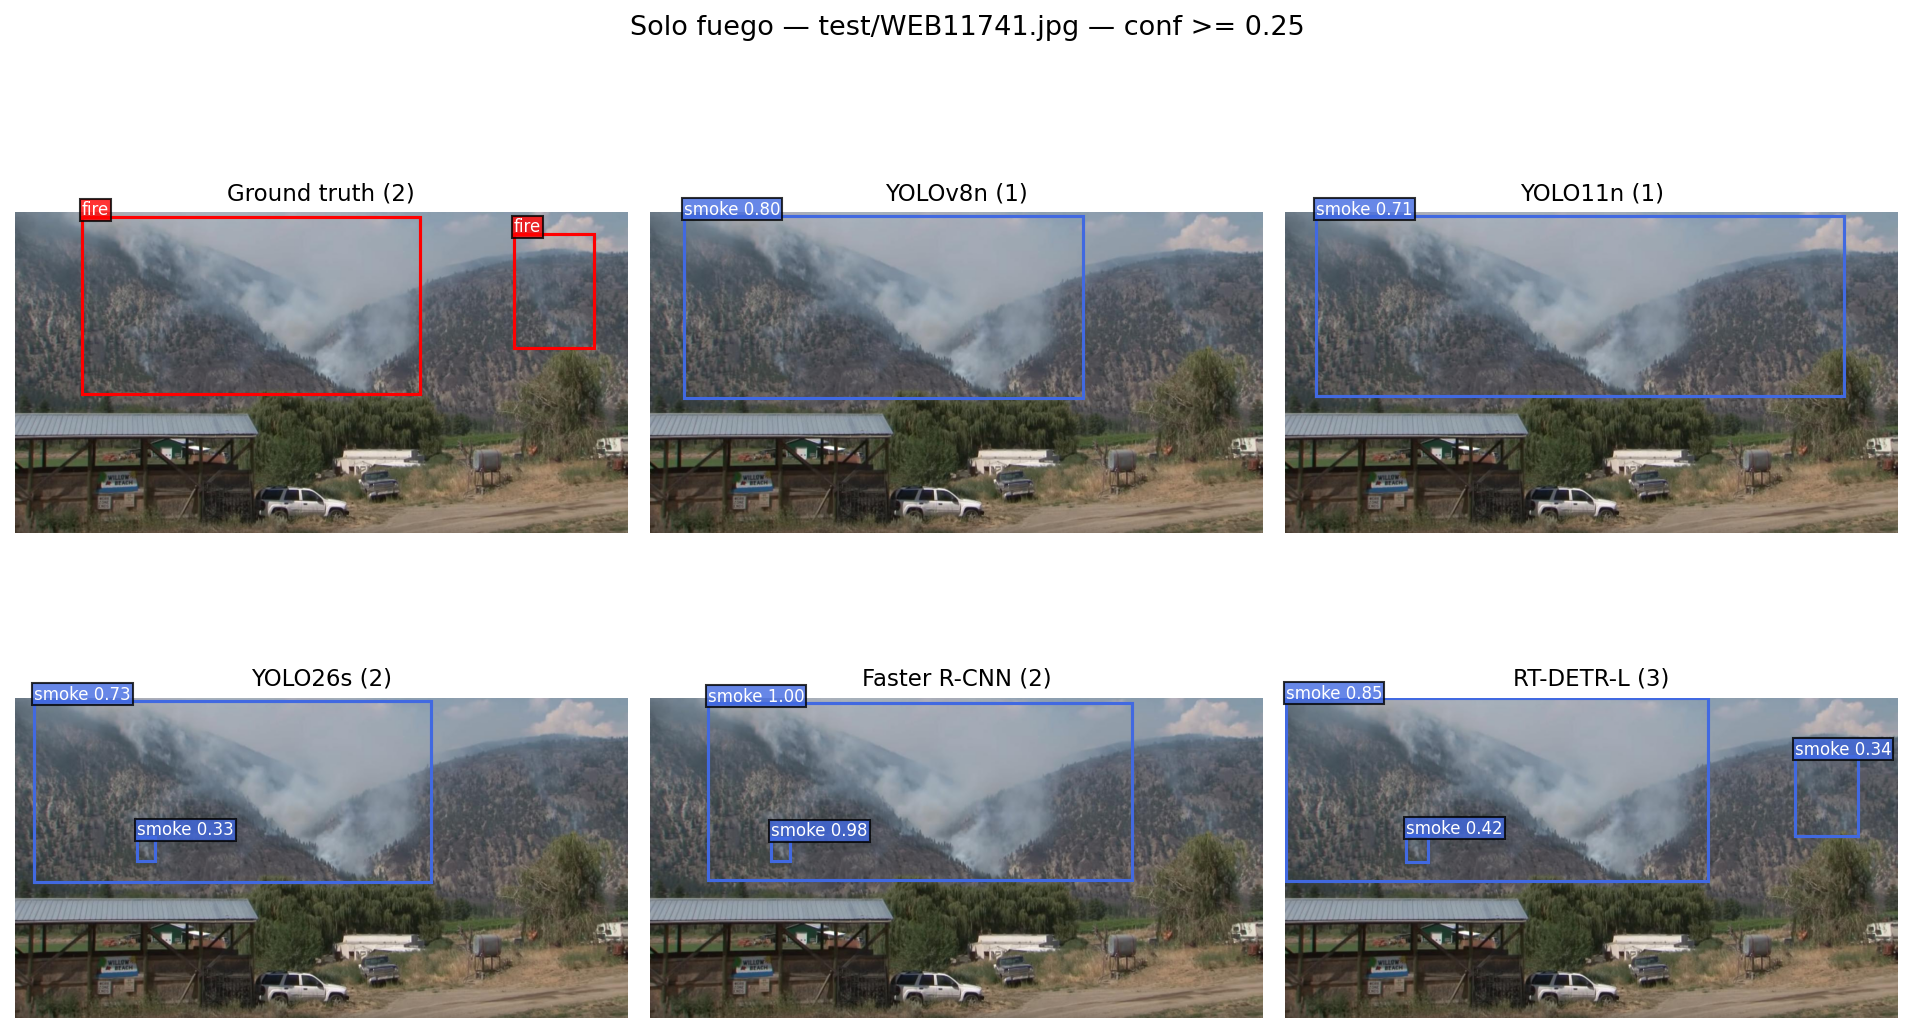
\includegraphics[width=0.7\textwidth]{cualitativa_solo_fuego_WEB11741.png}}
\caption{Error de anotación de origen (test/WEB11741, confianza $\geq 0.25$):
el ground truth etiqueta como \textit{fire} dos regiones que contienen humo.
Los cinco modelos predicen \textit{smoke} sobre esas regiones, contradiciendo
la anotación pero describiendo correctamente la escena.}
\label{fig:cualitativa_etiqueta}
\end{figure*}

Finalmente, la Fig.~\ref{fig:cualitativa_etiqueta} documenta el efecto de los
errores de anotación mencionados en la Sección~\ref{Preparacion_datos}: el
ground truth etiqueta como \textit{fire} dos regiones que contienen humo, y
los cinco modelos coinciden en predecir \textit{smoke}. La evaluación
automática computa estos aciertos perceptuales como errores dobles (falso
negativo de \textit{fire} y falso positivo de \textit{smoke}): parte del
techo común de mAP observado es atribuible al ruido de las anotaciones y no
a limitaciones de los detectores.

Se observa además una diferencia sistemática en la calibración de las
confianzas: Faster R-CNN asigna valores cercanos a 1.0 a sus detecciones,
RT-DETR-L valores intermedios y los YOLO valores más conservadores
(típicamente entre 0.3 y 0.8), posiblemente influida por la capacidad de
cada modelo. Esta diferencia no afecta el mAP, pero sí es relevante en la
práctica: el umbral de alarma de un sistema en producción debe calibrarse
por modelo y no puede transferirse de una arquitectura a otra.


% ============================================================
% IV. CONCLUSIONES
% ============================================================

\section{Conclusiones}

Del trabajo realizado se extraen las siguientes conclusiones:

\begin{enumerate}

\item \textbf{La elección de arquitectura no es el factor dominante del
desempeño.} Cinco modelos que difieren en paradigma y en más de un orden de
magnitud en parámetros convergen a un rango de 2.1 puntos en mAP@0.5 (0.757
a 0.778). El techo común, junto con la evidencia de errores de anotación,
indica que la calidad del dataset condiciona el resultado más que la
capacidad del modelo, y que el esfuerzo de mejora debería dirigirse a los
datos antes que a arquitecturas más grandes.

\item \textbf{Los modelos livianos de una etapa ofrecen el mejor compromiso
para la aplicación.} YOLOv8n alcanza el 97\% del mejor mAP@0.5:0.95 con 3M
de parámetros y 455 FPS, 60 veces más rápido que Faster R-CNN, al que además
supera en mAP; YOLO26s obtiene el mejor mAP absoluto (0.778 y 0.459)
manteniendo 188 FPS. Para monitoreo de múltiples cámaras en tiempo real los
YOLO son la elección justificada por las métricas; Faster R-CNN solo se
justifica en procesamiento diferido, donde su F1 superior (0.761) y su
ventaja en objetos pequeños compensan su costo.

\item \textbf{El fuego es estructuralmente más difícil de detectar que el
humo.} La brecha de unos 10 puntos de mAP@0.5 entre clases (0.798--0.828
para \textit{smoke} frente a 0.709--0.725 para \textit{fire}) se repite en
los cinco modelos y se explica por el tamaño de las cajas de fuego,
mayoritariamente muy pequeñas. La evaluación cualitativa confirma que los
objetos diminutos son el punto ciego de los YOLO livianos; aumentar la
resolución de entrada o la capacidad del modelo son las mejoras candidatas.

\item \textbf{El error dominante es la omisión, no la confusión entre
clases.} La confusión \textit{smoke}--\textit{fire} es del orden del 1\%,
mientras que las instancias no detectadas alcanzan el 21\% en humo y el 29\%
en fuego (YOLOv8n). Dado que el falso negativo es el error más costoso en
alerta temprana, la principal línea de mejora es el recall; la ausencia de
falsos positivos observada en escenas negativas sugiere margen para operar
con umbrales más bajos.

\item \textbf{Las métricas constituyen una cota con doble sesgo y deben
interpretarse con cautela.} La partición a nivel de imagen de secuencias
temporales puede inflar optimistamente los resultados, mientras que los
errores de anotación penalizan predicciones perceptualmente correctas, como
el caso en el que los cinco modelos revierten una etiqueta errónea. Como
trabajo futuro se propone re-particionar el conjunto por cámara y secuencia,
depurar las anotaciones y repetir los entrenamientos con múltiples semillas
para dotar de significancia estadística a la comparación.

\end{enumerate}


% ============================================================
% REFERENCIAS
% ============================================================

\begin{thebibliography}{00}

\bibitem{b1}
J. Redmon, S. Divvala, R. Girshick, and A. Farhadi,
``You only look once: Unified, real-time object detection,''
in \textit{Proceedings of the IEEE Conference on Computer Vision and Pattern
Recognition},
pp. 779--788, 2016.

\bibitem{b2}
S. Ren, K. He, R. Girshick, and J. Sun,
``Faster R-CNN: Towards real-time object detection with region proposal
networks,''
in \textit{Advances in Neural Information Processing Systems},
vol. 28, 2015.

\bibitem{b3}
Y. Zhao, W. Lv, S. Xu, J. Wei, G. Wang, Q. Dang, Y. Liu, and J. Chen,
``DETRs beat YOLOs on real-time object detection,''
in \textit{Proceedings of the IEEE/CVF Conference on Computer Vision and
Pattern Recognition},
pp. 16965--16974, 2024.

\bibitem{b4}
P. V. A. B. de Venâncio, A. C. Lisboa, and A. V. Barbosa,
``An automatic fire detection system based on deep convolutional neural
networks for low-power, resource-constrained devices,''
\textit{Neural Computing and Applications},
vol. 34, pp. 15349--15368, 2022.

\bibitem{b5}
G. Jocher, A. Chaurasia, and J. Qiu,
``Ultralytics YOLO,'' 2023.
\texttt{https://github.com/ultralytics/ultralytics}

\end{thebibliography}

\end{document}
